\begin{figure}[htbp]
    \centering
    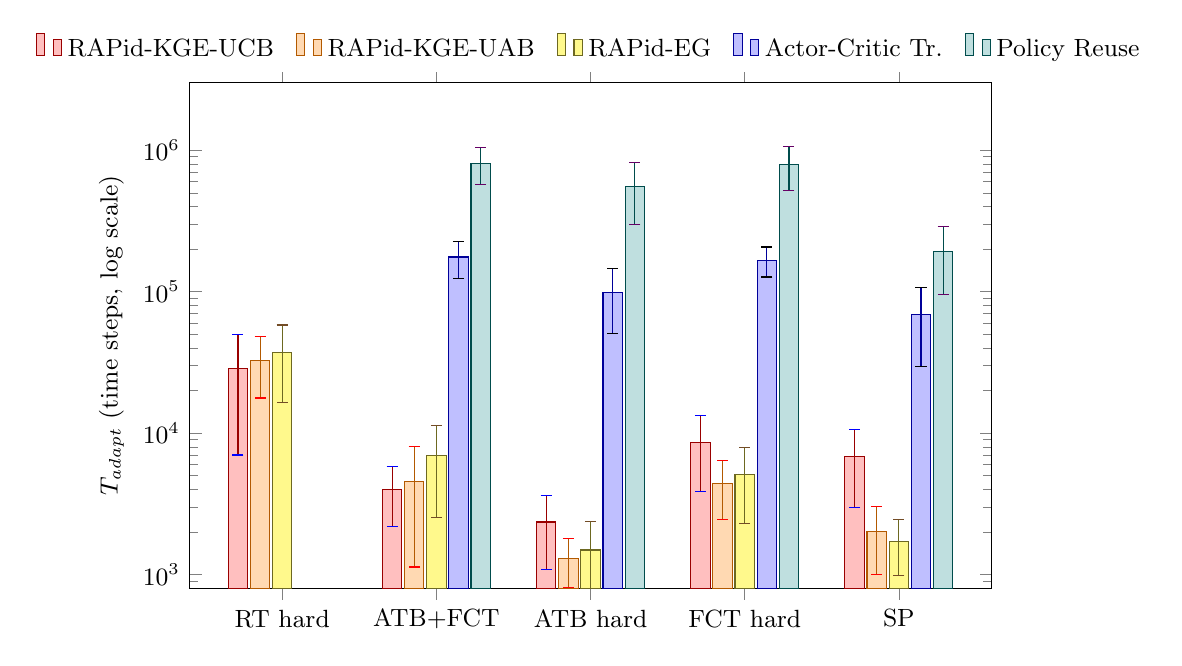
\begin{tikzpicture}
    \begin{axis}[
        ybar=1pt,
        bar width=7pt,
        width=0.97\textwidth, height=8cm,
        enlarge x limits=0.15,
        ymode=log,
        log origin=infty,
        ymin=800, ymax=3000000,
        ylabel={$T_{\text{adapt}}$ (time steps, log scale)},
        symbolic x coords={RT hard, ATB+FCT, ATB hard, FCT hard, SP},
        xtick={RT hard, ATB+FCT, ATB hard, FCT hard, SP},
        legend style={at={(0.5,1.02)}, anchor=south, legend columns=5,
                      font=\small, draw=none, /tikz/every even column/.append style={column sep=6pt}},
        error bars/y dir=both, error bars/y explicit,
        tick label style={font=\small},
        label style={font=\small},
    ]
    % RAPid-KGE-UCB
    \addplot+[draw=red!60!black, fill=red!25] coordinates {
        (RT hard,28500) +- (0,21500) (ATB+FCT,4020) +- (0,1820)
        (ATB hard,2350) +- (0,1270) (FCT hard,8610) +- (0,4730)
        (SP,6820) +- (0,3830) };
    % RAPid-KGE-UAB
    \addplot+[draw=orange!70!black, fill=orange!30] coordinates {
        (RT hard,32800) +- (0,15100) (ATB+FCT,4560) +- (0,3430)
        (ATB hard,1300) +- (0,489) (FCT hard,4400) +- (0,1960)
        (SP,2010) +- (0,1010) };
    % RAPid-EG
    \addplot+[draw=olive!70!black, fill=yellow!45] coordinates {
        (RT hard,37300) +- (0,20800) (ATB+FCT,6930) +- (0,4410)
        (ATB hard,1490) +- (0,865) (FCT hard,5120) +- (0,2840)
        (SP,1720) +- (0,738) };
    % Actor-Critic Transfer (did not converge on RT hard)
    \addplot+[draw=blue!60!black, fill=blue!25] coordinates {
        (ATB+FCT,176000) +- (0,51300)
        (ATB hard,98000) +- (0,47500) (FCT hard,167000) +- (0,39900)
        (SP,68600) +- (0,38900) };
    % Policy Reuse (did not converge on RT hard)
    \addplot+[draw=teal!60!black, fill=teal!25] coordinates {
        (ATB+FCT,808000) +- (0,238000)
        (ATB hard,557000) +- (0,259000) (FCT hard,790000) +- (0,270000)
        (SP,193000) +- (0,97600) };
    \legend{RAPid-KGE-UCB, RAPid-KGE-UAB, RAPid-EG, Actor-Critic Tr., Policy Reuse}
    \end{axis}
    \end{tikzpicture}
    \caption[Adaptation time of \RAPidLearn{} and transfer-learning baselines]{Bar-chart visualization of the adaptation time ($T_{\text{adapt}}$, lower is better, log scale) reported in \cref{tab:rapid_learn_results}. Error bars denote one standard deviation over 10 independent trials. All \RAPidLearn{} variants (KGE-UCB, KGE-UAB, EG) adapt one to two orders of magnitude faster than the transfer learning baselines. Transfer learning baselines did not converge on the RT hard scenario and are omitted from that group.}
    \label{fig:rapid_learn_results_bars}
\end{figure}
